\chapter{Testing with System Models}
\label{sec:topic_7}

In this chapter, we aim to study the topic \textit{testing with  system models}. Section \ref{sec:Intro7} presents the introduction of this topic. Section \ref{sec:LS} describes how the systematic literature research is carried out to identify the existing approaches for testing with system models. In \autoref{sec:AP1}, the first relevant approach for this topic, which is given from the Chair of Software Engineering of University Heidelberg to be studied, is described and implemented on the example application \textit{Movie Manager}. In \autoref{sec:AP2}, the second relevant approach, which is identified through the literature research, is studied likewise. Then, \autoref{sec:Compar} compares the two relevant approaches selected for this topic. In conclusion, \autoref{sec:Conc} presents the insights gained from this study.

In order to get familiar with \textit{system model (SM), test model (TM), system under test (SUT), model-based testing (MBT), Unified Modeling Language (UML), Systems Modeling Language (SysML)} and \textit{Object Constraint Language (OCL)}, please visit the glossary.


\section{Introduction}
\label{sec:Intro7}

The key to successful product engineering in the software industry today is in many cases a good quality-assurance and deployment of software systems \cite{Paper1}. In order to ensure the quality of a product and verify that the product meets its requirements, we need software testing. 

Model-based testing (MBT) is a software testing technique that has gained much interest in recent years by providing the degree of automation needed for shortening the time required for testing \cite{Paper1}. It provides automatic generation of tests from models representing the behavior of the system under test (SUT) \cite{matera}. From these models, test cases can be derived directly or via some model transformations following different coverage criteria. 

As our topic is testing with system models, it is important to differentiate the two model types \textit{system model} (SM) and \textit{test model} (TM) with respect to the MBT. In our first approach \cite{Paper1}, which is presented in \autoref{sec:AP1}, the authors explicitly stated that they used SMs instead of TMs. And the difference between SM and TM is explained as follows: \enquote{The difference between the two being that the former is both used for development and testing, whereas the latter is only used for testing} \cite{Paper1}. 

In order to discuss the differences between using SM and TM in particularly, the authors of \cite{Paper1} provide with some additional authors the article \textit{Model-Based Testing using System vs. Test Models – What is the Difference?} \cite{SMvsTM}, which is newer than \cite{Paper1} and presents two model-based testing case study examples which use SMs and TMs, respectively. In \cite{SMvsTM}, the SM case study example is our first approach \cite{Paper1} to be studied within this chapter.

The article \cite{SMvsTM} summarizes the differences between the SMs and TMs as shown in \autoref{fig:smtm}.

\begin{figure} [H] 
\centering
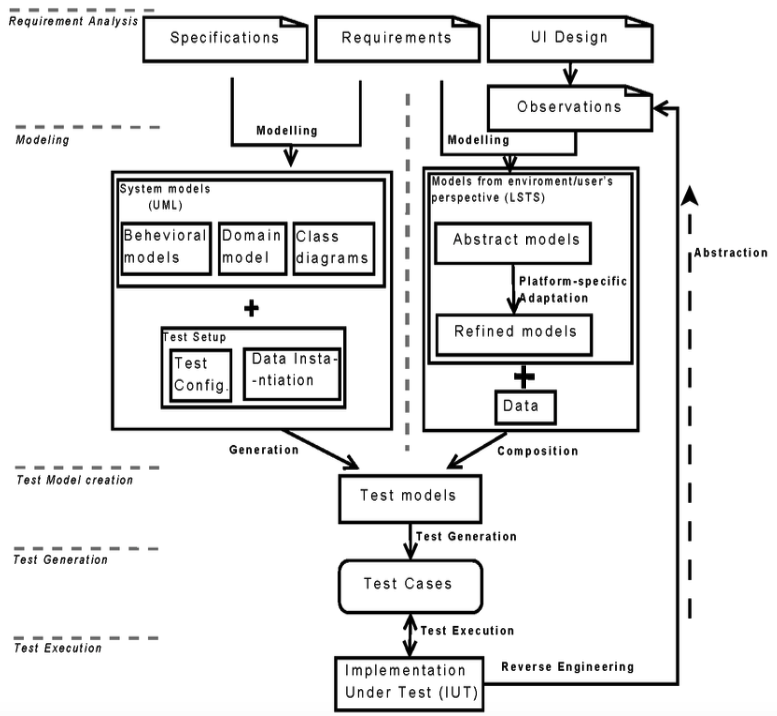
\includegraphics[scale=0.35]{../images/smtm} 
\caption{Sytem models and test models}
\label{fig:smtm}
\end{figure}

From the viewpoint of modeling, one difference between SM and TM is in the way the expected behavior of the SUT is specified with respect to its interfaces; SM provides an internal viewpoint, whereas the TM provides an external viewpoint of the SUT \cite{SMvsTM}. In the terms of reactive systems, TMs provide stimuli and observe the SUT reactions, while the SMs expect the stimuli and provide reactions. Concerning the purpose of modeling, the TMs are developed solely for testing while SMs can be primarily developed for system development (however, SMs are simpler and more abstract than implementation models) and then used for testing as well \cite{SMvsTM}. \\
However, there also some definitions in \cite{SMvsTM}, which conflict with the usage and the way of the models are created in \cite{Paper1}. According to \cite{SMvsTM}, in TM based approaches, implementation is seen as a black-box thus it is hard to give any verdict about how much of the implementation code has been covered by generated test cases unless source code is instrumented for this purpose. Therefore, requirement coverage is mostly used in this case. On the other hand, in SM based approaches, both code and requirement coverage can be observed, again provided that the implementation code is available for such analysis. \\
But as can be seen in \autoref{sec:AP1}, the authors are entirely concerned with the requirement coverage in \cite{Paper1} while using SMs. After stating this, we would like to clarify that for our study we stick to the definition and usage of SM provided in \cite{Paper1}, as it is also suitable with the \autoref{fig:smtm}.

As the SM of the SUT is typically derived from the informal requirements, it is important to trace how different requirements reflect in the models, on different perspectives and on different abstraction levels, and how the generated test cases cover different requirements \cite{Paper1}, \cite{SMvsTM}. For a model-based testing perspective, traceability of requirements means that the generated test cases from the model are linked with the requirements \cite{Paper2}. Thus, traceability of requirements helps to achieve the right level of coverage and shows what requirement has been covered by what test \cite{Paper1}. It also enables us to identify which requirements have been successfully tested and which have resulted in failures \cite{Paper1}. Hereby, traceability of requirements is a pivotal aspect of MBT that allows one to ensure that all requirements have been tested  \cite{matera}.

%\newpage
\section{Literature search}
\label{sec:LS}

This section describes the systematic literature research carried out according to the \textit{Guidelines for Literature Research of the Chair of Software Engineering} \cite{LRGuidelines}. It aims to identify and analyze the scientific articles regarding testing with system models. 

\subsection*{Research question and research strategy}
\label{subsec:RQ}
The main goal of this search is to find relevant approaches for testing with system models, which are similar to the approach provided in the given article \textit{Tracing Requirements in a Model-Based Testing Approach} \cite{Paper1}. 

Based on \cite{Paper1}, which is our start paper for \autoref{sec:topic_7} in this study, we derive the following research question presented in \autoref{tab:RQ}.

\begin{table} [htb] 
\centering
\begin{small}
\caption{Research question and search terms}
\label{tab:RQ}
\setlength{\tabcolsep}{1em}
\begin{tabular}{ l| p{10cm}}
\hline
\textbf{Research Question} & Which approaches exist to generate test cases using system models for the traceability of requirements?\\
\hline
\textbf{Search Terms}  & system model* AND test* AND trac* AND requirement? \\
\hline
\end{tabular}
\end{small}
\end{table}

In order to answer the research question and find relevant articles, we use \enquote{keyword-based search} and \enquote{snowballing} methods. For the keyword-based search method, we determined the search terms as presented in \autoref{tab:RQ}. These search terms were derived from the research question to focus on a certain aspect of the given article \cite{Paper1} and to find a similar approach. 

For the literature research, the digital libraries of the IEEE Xplore (Institute of Electrical and Electronics Engineers)\footnote{IEEE Xplore \url{https://ieeexplore.ieee.org}} and ACM (Association for Computing Machinery)\footnote{ACM Digital Library \url{https://dl.acm.org}} were used as main sources, since they include the most extensive range of examined scientific publications and are widely recognized. 

In this literature research, keyword-based search method and snowballing search method are conducted to find relevant articles in aforesaid libraries. With keyword-based search method, we search for the search terms presented in \autoref{tab:RQ} with different combinations, since each digital library has a different search method, e.g.  advanced search, or command search.

Snowballing search method is applied to the given article \cite{Paper1} to identify further relevant articles. With backward snowballing method, we go through the reference list of \cite{Paper1} and select the articles as relevant, which fulfill the relevance criteria determined during the literature research. The relevance criteria are presented in \autoref{tab:ArticleCriteria}. With forward snowballing method, we go through the articles, which cite the given article, and again select the articles as relevant, if they fulfill the relevance criteria.

%\subsection{Research Strategy}
%\label{subsec:RS}

\begin{table} [htb] 
\centering
\begin{small}
\caption{Criteria for selecting an article as relevant}
\label{tab:ArticleCriteria}
\setlength{\tabcolsep}{1em}
\begin{tabular}{ l| p{12cm}}
\hline
\textbf{No.} & \textbf{Description} \\
\hline
1 & The article is available in English\\
\hline
2  & The article has a clear focus on software engineering\\
\hline
3  & The article was published in the last fifteen years (2005-2020) \\
\hline
4  &  The article contains an approach for the traceability of requirements using system models to generate test cases, i.e. the article answers the research question\\
\hline
\end{tabular}
\end{small}
\end{table}

In order to ensure that the research methodology and its implementation remain consistent and comprehensible, we formulated four relevance criteria as shown in \autoref{tab:ArticleCriteria}. An article is relevant, if it fulfills all criteria. The first two criteria are formulated to check the availability and the subject area of the articles. Since this work is to be written in English, the article to be used should be available in English. To reduce the comprehensive subject area to the relevant area for our topic, the article should have a clear focus on the area of software engineering as described in the second criterion. The third criterion aims to focus on recent work and to limit the search results. The last criterion is formulated to answer the research question and to find relevant articles, which particularly provide similar approaches to the approach presented in \cite{Paper1}.

\subsection*{Research execution and literature results}
\label{subsec:RE}

First, the search was carried out using the keyword-based search method with aforesaid search terms. In \autoref{tab:ResultKeyword}, the results of this search are documented.\\
First column shows the search location, second column shows the date on which the search was carried out, and third column shows the applied restriction of search. Fourth column presents the exact search query of the search terms and thus shows how they were searched in the specified parts of articles. Fifth column shows the number of overall results, and sixth column shows the number of relevant articles. Finally, last column presents the number of articles chosen to be used in this study.

\begin{table} [H] 
\begin{small}
  \begin{center}
  \begin{scriptsize}
\caption{Results of the keyword-based search method}
\label{tab:ResultKeyword}
\begin{tabular}{   m{1cm} | m{1cm} | m{1.6cm} | m{4.8cm} | m{1cm} | m{1.2cm} | m{0.7cm}  }
\hline
\textbf{Search Location} & \textbf{Search Date} & \textbf{Restriction}  & \textbf{Search Terms}  &  \textbf{\# Results}  & \textbf{\# Relevant Articles}  &  \textbf{Used Results} \\
\hline
IEEE & 20.11.20 & 2005-2020, Advanced Search & ((((\enquote{Full Text Only}:\enquote{system model*}) AND \enquote{Document Title}:test*) AND \enquote{Abstract}:trac*) AND \enquote{Full Text Only}:requirement?) & 64 & 2 & 0\\
\hline
ACM & 20.11.20 & 2005-2020, Advanced Search & $[$Full Text: \enquote{system model*}$]$ AND $[$Publication Title: test* $]$ AND $[$Abstract: trac*$]$ AND $[$Full Text: requirement?$]$ AND $[$Publication Date: (01/01/2005 TO 12/31/2020)$]$ & 9 & 0 & 0\\
\hline
ACM & 21.11.20 & 2005-2020, Advanced Search & $[$Abstract: system model*$]$ AND $[$Publication Title: test*$]$ AND  $[$Abstract: trac*$]$ AND $[$Abstract: requirement?$]$ AND $[$Publication Date: (01/01/2005 TO 12/31/2020)$]$ & 46 & 2 & 0 \\
\hline
IEEE & 21.11.20 & 2005-2020, Advanced Search & ((((\enquote{Abstract}:system model*) AND \enquote{Abstract}:requirement?) AND \enquote{Abstract}:trac*) AND \enquote{Document Title}:test*) & 59 & 0 & 0\\
\hline
\end{tabular}
\end{scriptsize}
 \end{center}
\end{small}
\end{table}
\newpage
As shown in \autoref{tab:ResultKeyword}, in all of our searches we searched the search term \enquote{test*}  in the \textit{documentation title} part, and the search term \enquote{trac*} in the \textit{abstract} part of the digital libraries, in order to find the closest approaches as possible to the presented approach in \cite{Paper1}. Although the \enquote{system model} is the most important search term for this topic, it was not written even in the abstract of the given article \cite{Paper1}. Therefore, with considering that, we decided to search this term also in the \textit{full text} part, instead of only in the \textit{abstract} part of the digital libraries. Consequently, the search terms \enquote{system model} and \enquote{requirement} were searched in the first searches only in \textit{full text} part, then in the second searches in \textit{abstract} part of the digital libraries. 

After identifying relevant articles by using keyword-based search method, snowballing method was conducted to the \cite{Paper1}, which is our start paper for this study, in order to find further relevant articles. The results of the search using snowballing method are detailed documented in \autoref{tab:ResultSnowballing}.

\begin{table} [H] 
\begin{small}
\begin{center}
\begin{scriptsize}
\caption{Results of the snowballing search method}
\label{tab:ResultSnowballing}
\begin{tabular}{  m{1.2cm} | m{4.7cm} | m{1.3cm} | m{1.6cm} | m{1.7cm} | m{1.2cm} }
\hline
\textbf{Search Date} & \textbf{Reference} & \textbf{Direction}  & \textbf{Number of Citations}  &  \textbf{\# Relevant Articles}  &  \textbf{Used Results} \\
\hline
\multirow{2}{1.2cm}{19.11.20} &  \multirow{2}{4.7cm}{\cite{Paper1} Tracing Requirements in a Model-Based Testing Approach} & Backward & 15 &  1 &1  \\ \cline{3-6} & & Forward &11 &1 & 0\\ 
\hline
\end{tabular}
\end{scriptsize}
 \end{center}
	\end{small}
\end{table}

Thus, after conducting the keyword-based and snowballing search methods, we could identify six relevant articles presented in \autoref{tab:RelevantArticles}.

\begin{table} [H] 
	\begin{small}
  \begin{center}
  \begin{scriptsize}
\caption{Results of the literature search}
\label{tab:RelevantArticles}
\begin{tabular}{  m{0.5cm} | m{4.7cm} | m{4.6cm} | m{1.2cm} | m{1.2cm}  }
\hline
\textbf{ID} & \textbf{Title} & \textbf{Authors} & \textbf{Year}  & \textbf{Source}  \\
\hline
\cite{Paper1}&Tracing Requirements in a Model-Based Testing Approach & F. Abbors, D. Truscan and J. Lilius, & 2009 & IEEE \\
\hline
\cite{matera}& MATERA - An Integrated Framework for Model-Based Testing& F. Abbors, D. Truscan and A. Baecklund & 2010 & IEEE\\
\hline
\cite{Relevant3} & A Subset of Precise UML for Model-Based Testing &F. Bouquet, C. Grandpierre, B. Legeard, F. Peureux, N. Vacelet, and M. Utting&2007&ACM \\
\hline
\cite{Relevant4}& Requirements Traceability in Automated Test Generation - Application to Smart Card Software Validation & F. Bouquet, E. Jaffuel, B. Legeard, F. Peureux, and M. Utting&2005&ACM \\
\hline
\cite{SMvsTM} & Model-Based Testing using System vs. Test Models – What is the Difference? &  F. Abbors, D. Truscan, J. Lilius, M. Katara, H. Virtanen, A. Jaeaeskelaeinen, and Q. A. Malik& 2010&IEEE\\
\hline
\cite{Paper2} & Requirements Traceability in the Model-Based Testing Process &Eddy Bernard and Bruno Legeard & 2007&DBLP\tablefootnote{dblp computer science bibliography \url{https://dblp.uni-trier.de/}} \\
\hline
\end{tabular}
\end{scriptsize}
 \end{center}
\end{small}
\end{table}
The articles \cite{Paper1}, \cite{matera}, \cite{Relevant3}  and \cite{Relevant4} were identified through the keyword-based search method, and \cite{SMvsTM} and \cite{Paper2} were identified through the snowballing search method. The first identified article \cite{Paper1} through the keyword-based search method was already given us for this study as start paper. Since \cite{matera} and \cite{SMvsTM} are from the same author group of \cite{Paper1}, we didn't choose them for our study as a second approach to examine. 

The articles \cite{Relevant3} and \cite{Relevant4} have also common authors, and one of them is the same author of the article \cite{Paper2}. Therefore, we excluded the \cite{Relevant3} and \cite{Relevant4}, and chose only \cite{Paper2}, \textit{Requirements Traceability in the Model-Based Testing Process}, which is closest to the provided approach in the given article \cite{Paper1}, and very suitable for our topic \textit{testing with system models}.

Consequently, \textbf{\textit{Tracing Requirements in a Model-Based Testing Approach}} \cite{Paper1} and \textbf{\textit{Requirements Traceability in the Model-Based Testing Process}}  \cite{Paper2} are the chosen articles to be studied in this \autoref{sec:topic_7}.


\section{Approach 1: Tracing Requirements in a Model-Based Testing Approach}
\label{sec:AP1}

This section describes the approach presented in \textit{Tracing Requirements in a Model-Based Testing Approach} \cite{Paper1}, and its application on the \textit{Movie Manager}, which is an application used by private individuals at home to manage their own film collection \cite{MovieManager}. What this management includes is described as sub-tasks in the user task sheet of Movie Manager in \cite{MovieManager}. 

\subsection{Description}
\label{subsec:DE1}
This approach was presented in 2009 by Fredrik Abbors, Dragos Truscan, and Johan Lilius in \cite{Paper1} for tracing product requirements across a model-based testing process. With this approach, the authors show how the informal requirements of the SUT evolve and are traced to system specifications and from system specification to tests during the test generation process. They also show how the test results are analyzed and traced back the specification of the system. 
%The approach is only described using small examples from a telecommunications case study. In that case, the SUT is a mobile switching server (MSS), which is a network element located in a mobile telecommunication system. The MSS is responsible for keeping track of the location of mobile subscribes (MS) in the network and for connecting calls between MS’s over 2G and 3G networks. The MSS is also responsible for tracking the movement of MS’s during an ongoing call\\
%Figure~\ref{fig:Ap1-1} presents the model-based testing process of this approach.\\

\begin{figure} [h] 
\centering
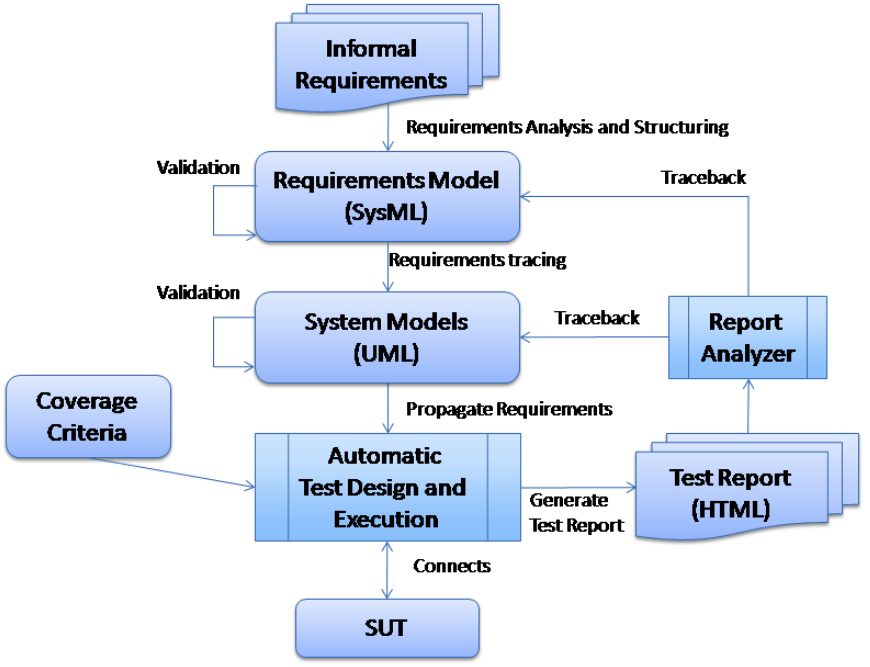
\includegraphics[scale=0.25]{../images/Ap1-1.png} 
\caption{Overview of the model-based testing process \cite{Paper1} }
\label{fig:Ap1-1}
\end{figure}

As shown in \autoref{fig:Ap1-1}, the model-based testing process starts with the analysis and structuring of the informal requirements (including protocol specifications, standards, user scenarios, etc.) into a \textit{requirements model} via Systems Modeling Language (SysML). Because compared to the pure textual description of requirements, a requirement diagram offers several advantages due to its visual overview, e.g. missing aspects can be easily identified to help identify additional requirements, and the different types of relationships facilitate traceability and promote understanding \cite{netreqdia}. Requirements traceability is built on top of this testing process, since authors want to be able to trace how different parts of the system models relate to the requirements and then to see how different requirements are covered by the generated test cases. Another reason for tracing requirements is that if a requirement changes, it is essential to know how this change is reflected in the models. Therefore, after requirements are structured hierarchically using SysML requirements diagrams, they are traced to different models or parts of the models implementing them. 
 
%Secondly, once the test report becomes available, we would like to be able to identify which requirements have been successfully tested and which have resulted in failures. In addition, for the failed test cases we should be able to trace back from test cases those parts of the SUT specification that generated the failure.
For the modeling, the Unified Modeling Language (UML) is used to specify the SUT. For a successful test derivation, several perspectives of the SUT are modeled; a class diagram is used to specify a \textit{domain model}, a \textit{behavioral model} is used to describe the behavior of the SUT, \textit{data models} are used to describe the message types exchanged between different domain entities, and \textit{domain configuration models} are used to represent specific test configurations using object diagrams. In order to increase the quality of the resulting models, a set of modeling guidelines and validation rules are defined. These rules ensure that the models are consistent with each other and moreover, that they contain the information needed in the later phases of the testing process. For editing the SysML and UML models and for running these validation rules, the NoMagic’s \textit{MagicDraw}\footnote{NoMagic MagicDraw \url{https://www.nomagic.com/products/magicdraw}} tool has been used. 

When all requirements have been linked to model elements and the models have been validated, the models used to specify the SUT are subsequently transformed into input for an automated test derivation tool for model driven testing, \textit{Conformiq Qtronic}\footnote{Conformiq Qtronic \url{https://www.conformiq.com/}}, via an automated transformation. Qtronic accepts as input a SM of the SUT from which it automatically designs test cases according to the selected coverage criteria. The input model can be expressed as a combination of UML state machines \cite{SMvsTM} and the transformation basically translates these UML models to the Qtronic Modeling Language (QML), a textual specification language with a Java-like syntax used by Qtronic for specifying the SUT. There are two main purposes for modeling behavior using state machines. First, by using UML state machines the behavioral properties of SUT specification are formally verified. Second, Qtronic tool expects the behavior of SUT in the form of state machines \cite{traqml}. During the transformation from UML to QML, links between requirements and model elements are preserved. 

In this approach, only the online testing mode of this Qtronic is used, in which tests are generated and applied on-the-fly against the SUT. For test generation, different coverage criteria types can be manually selected from the graphical user interface (GUI) of Qtronic like requirements, state, transitions, paths, conditional, or statement coverage. The generated test cases are sequences of input/output messages and their data values derived from the SMs to be sent/received by the SUT \cite{SMvsTM}. As the designed test cases are at the same abstraction level as the SM, an adapter is used to concretize the tests \cite{SMvsTM}. One-by-one Qtronic generates an input message, sends it via the adapter to the SUT, and generates a new input message based on the responses from the SUT. A logging back-end can be used during test execution. The logging back-end provides connectivity to the Qtronic reporting infrastructure and it is used by Qtronic to generate a test report. Three logging back-ends are provided by default. With these logging back-ends, Qtronic can generate test reports in HTML, SQLite, and XML format. When all tests have been applied against the SUT, Qtronic generates a test report in the chosen format, which summarizes the results of the testing process in terms of generated test cases, verdicts, coverage levels, requirements traceability matrix, etc. Unfortunately, the rest of the automatic test generation and execution process of this approach was not provided by the authors. 

With this approach, it is also possible to trace-back requirements from test cases to models. For this purpose, the rest report is analyzed and the information of the failed test cases is collected. Then, the requirements attached to those test cases are traced back to system models. This enables to identify which requirements were not validated during testing and to what parts of the specification they are linked. A Python script was developed by the authors that automatically analyzes the Qtronic test report. 

According to the authors, the provided approach proved beneficial through the fact that many errors have been detected in the early stages of the process, when the system models have been created. For instance \cite{SMvsTM}, some errors originated from inconsistencies discovered in the SM, which were due to misunderstanding of requirements or to incomplete validation of models before testing. Other errors have been found in the adapter, as well as in the SUT.

Furthermore, it should be noted that although Conformiq is still active and offering different kind of products for an end-to-end test automation, its Qtronic product mentioned in this approach is not existing in Conformiq's current product list. Unfortunately, after our research, we could not find any information about what happened to Qtronic. Therefore, we assume that it was not developed further.





\subsection{Application}

%As presented in Figure~\ref{fig:Ap1-s1}, 
First, functional requirements of the SUT should be analyzed and structured into requirements models using the requirements diagrams of SysML. Each requirement element contains a \textit{name} field which specifies the name of the requirement, an \textit{id} field that simply specifies the id of the requirement, a \textit{text} field which describes the requirement, and a \textit{source} field which specifies the origins of the requirement. The source can be a link to or a name of a textual document from where the requirement has been extracted. 

In our implementation, we converted the user sub-tasks of Movie Manager into system functions in order to build a requirements diagram from system functional requirements. \autoref{fig:Ap1-req} presents the example of a SysML requirements diagram for our application. 


\begin{figure} [h] 
\centering
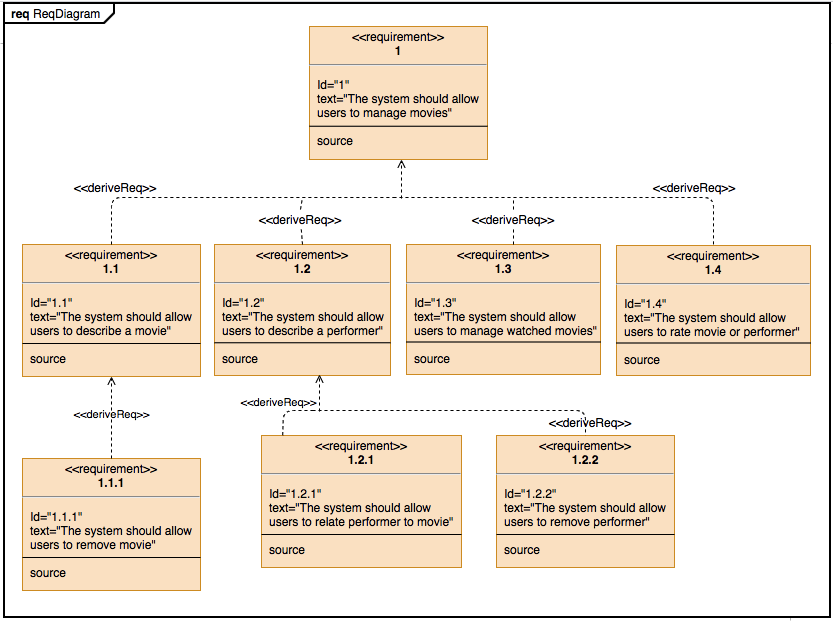
\includegraphics[scale=0.49]{../images/Ap1-req} 
\caption{Example of a SysML requirements diagram}
\label{fig:Ap1-req}
\end{figure}

%As presented in Figure~\ref{fig:Ap1-s2}, 
Then, the UML models of the SUT are built starting from the requirements models. During this process, the requirements should be traced to different parts of the models to point how each requirement is addressed by the models. In the provided approach, a set of modeling guidelines and validation rules should be defined for ensuring the quality of the resulting models. For this purpose, Object Constraint Language (OCL) is used. The aforementioned NoMagic’s MagicDraw tool has been used for editing the SysML and UML models and for running the validation rules. But in our implementation of the approach, we use the free online tool of the diagram software \textit{draw.io}\footnote{draw.io \url{https://drawio-app.com/}} via \textit{diagrams.net}\footnote{diagrams.net \url{https://www.diagrams.net/}} for this purpose.
\newpage
As the next step, a state machine model should be modeled from the requirements model, which is to be used as input for Qtronic, since the Qtronic tool expects the behavior of SUT in the form of state machines in order to be able to convert it into QML. %In the provided approach, the relationships between requirements and models are specified on several levels. For instance, non-leaf requirements are linked to state machine models, and leaf requirements in the requirements tree are linked to other UML elements to which they apply, e.g. transitions in a state machine or classes in a class diagram. As an exceptional situation, the top-level functional requirements are linked to use cases in the use case model of the SUT. \\
In \autoref{fig:Ap1-sm2}, we present an example for the requirement with the requirement id \enquote{1.4} from the requirements model presented in \autoref{fig:Ap1-req}.

\begin{figure} [H] 
\centering
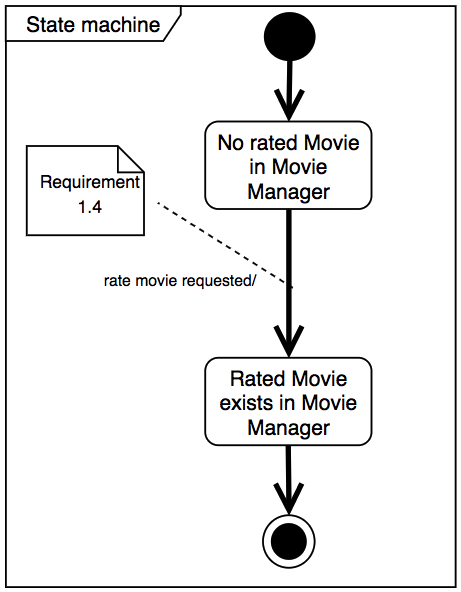
\includegraphics[scale=0.3]{../images/Ap1-sm2} 
\caption{Example of a UML state machine}
\label{fig:Ap1-sm2}
\end{figure}

But as already mentioned in the description of this approach in ~\autoref{subsec:DE1}, Qtronic is no longer available and therefore we can not apply the remaining steps, which are \textit{automatic test design and execution} and \textit{generation of test report}. As we could not find any information on how Qtronic generates tests, we can not provide any exemplarily test cases either. 




\section{Approach 2: Requirements Traceability in the Model-Based Testing Process}
\label{sec:AP2}

This section describes the approach presented in \textit{Requirements Traceability in the Model-Based Testing Process} \cite{Paper2}, and its application on Movie Manager. 

\subsection{Description}
\label{subsec:DE2}
This approach was presented in 2007 by Eddy Bernard and Bruno Legeard in \cite{Paper2} to automatically produce the traceability matrix from requirements to test cases, as part of the test generation process. Automatically generating the traceability matrix from requirements to test cases implies managing the links between the requirements specification, the model and the test cases. This approach focuses on this problem and is embedded in the \textit{LEIRIOS Test Designer} technology, which is named currently \textit{Smartesting}\footnote{Smartesting \url{https://www.smartesting.com/}} \cite{matera}. The approach tags the dynamic part of the UML model with the requirement identifiers and uses it to produce automatically both the test cases and the traceability matrix. 

First, the validation engineer constructs the model from a textual specification. The goal of this step is to translate the description of the features of the tested system into a precise UML model of the expected behavior \cite{LTG}. The LEIRIOS Test Designer approach uses a subset of the UML 2.0 language with class diagrams, instance diagrams, state machine diagrams, and OCL expressions. While the OCL expressions within the class diagram formally describe the expected behavior of operations of a class using preconditions and postconditions, the OCL expressions within the state machine formalize guards and effects of transitions between the states. 

Then, requirements traceability is managed by tagging manually the postconditions of the operations and the effects of the transitions in the UML model with the requirements. The format uses ad-hoc comment symbols to associate a requirement with an OCL statement which will be involved into a test target during the generation of the test cases. Once the model is reasonably trustworthy, the generation of tests is steered by the validation engineer on the basis of test selection criteria. Test selection criteria are supported by the LEIRIOS Test Designer tool to control the choice of tests from all the possible tests that can be derived from the behavior UML model \cite{LTG}, e.g. transition-based coverage, decision-based coverage, and data-oriented coverage. It is important to notice that all these test selection criteria are related to models and define how well the generated test suite covers the model \cite{LTG}. 

The test generation method is provided by the LEIRIOS Test Designer tool. It consists in testing all the possible behaviors of the specification operations, by traversing the states of the system. This strategy is controlled by the previously defined test selection criteria. 
\newpage
This method is performed as follows:
%
\begin{itemize}[noitemsep]
  \item [--]Partitioning of the model operation to generate all the possible expected behaviors,
  \item [--]Computation of variable domain boundaries from each behavior (called test targets),
   \item [--] Generation of test cases obtained, for each test targets, by traversing the underlying reachability graph of the model from the initial state to reach a state satisfying a test target.
\end{itemize}
Operations are the internal actions that modify the system state during the computation of user actions. They are called from the action part of transitions in the state machine and their meaning is defined by OCL postconditions in the class diagram \cite{LTG}. 

A test case reaches a target, which involves OCL statements tagged with one or several requirement identifiers. Then, LEIRIOS Test Designer makes it possible to match a test with requirements during the generation of the test cases. In LEIRIOS Test Designer, a general framework to convert the generated test cases into executable scripts is also provided. The test script pattern is a source code file in the target language with some tags indicating where sequences of operation invocations have to be inserted. A traceability matrix is obtained after the tests are executed. For each requirement, the matrix gives the list of needed test cases to test it. 

In \cite{Paper2}, this presented approach is implemented on a simplified version of a drink vending machine controller, which is SUT, with \enquote{Buy a drink} scenario to illustrate the test generation process with LEIRIOS Test Designer. After expected functional requirements of the SUT are listed, it is modeled via a \textit{class diagram}, an \textit{instance diagram} and a \textit{state machine}. Expected behaviors are specified by transitions (either external or internal) and those transitions are triggered by a \textit{user event}, a \textit{guard} and an \textit{effect}. Requirements traceability is managed by tagging the effect of each transition with requirement identifiers. This link between the model and the requirements is used by the LEIRIOS Test Designer tool to produce the traceability matrix between generated test cases and requirements. At the end, from the SUT model, 12 test targets are generated, one for each transition, and 12 test cases are generated. 

Unfortunately, the approach lacks the detailed explanation on how the test cases are generated and converted to executable test scripts via LEIRIOS Test Designer tool.




\subsection{Application}

In this part, we aim to to follow the same steps of the approach on our Movie Manager example as similar as possible. 

First, we get the informal requirements of the system under test. To do that, we create use case diagram of Movie Manager using draw.io tool as shown in \autoref{fig:Ap2-2}. Our use case scenario: \enquote{User manages movies and corresponding performer data of a movie collection}.

\begin{figure} [H] 
\centering
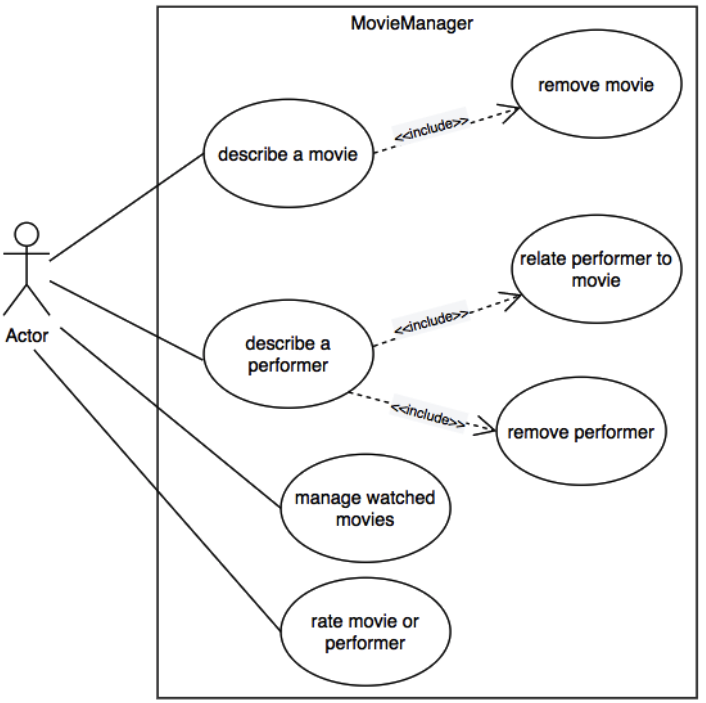
\includegraphics[scale=0.35]{../images/Ap2-2} 
\caption{Example for a use case diagram of Movie Manager}
\label{fig:Ap2-2}
\end{figure}

The system under test is the Movie Manager. To precisely define the expected functional requirements of the Movie Manager, a list of requirements including Req Identifier, Req Name, and Req description is defined as presented in \autoref{tab:MMreq}. For the requirements MM-2 and MM-7 we added some preconditions based on the Movie Manager \cite{MovieManager} to be able to apply the next steps of the approach within this section. 

\begin{table} [H] 
  \begin{center}
  \begin{small}
\caption{Movie Manager requirements}
\label{tab:MMreq}
\begin{tabular}{  m{1.3cm} | m{3.8cm} | m{8cm}  }
\hline
\textbf{Req. Id}& \textbf{Req. Name}&\textbf{Req. Description}   \\
\hline
MM-1& Describe\_Movie&The Movie Manager shall allow to describe a movie\\
\hline
MM-2&Remove\_Movie&The Movie Manager shall allow to remove movie. If the movie is linked with a performer, the user is warned by Movie Manager. The movie is removed from the database after user confirms.\\
\hline
MM-3&Describe\_Performer& The Movie Manager shall allow to describe a performer\\
\hline
MM-4&Relate\_Performer\_to\_Movie&The Movie Manager shall allow to relate performer to movie \\
\hline
MM-5&Remove\_Performer& The Movie Manager shall allow to remove performer\\
\hline
MM-6&Manage\_Watched\_Movies& The Movie Manager shall allow to manage watched movies\\
\hline
MM-7& Rate\_Movie\_or\_Performer& The Movie Manager shall allow to rate movie or performer. If the movie or performer does not exist, the user is warned by Movie Manager\\
\hline
\end{tabular}
\end{small}
 \end{center}
\end{table}

Then as an instance, we create the Movie Manager Class Diagram for the aforementioned requirements as presented in \autoref{fig:Ap2-class}.

\begin{figure} [H] 
\centering
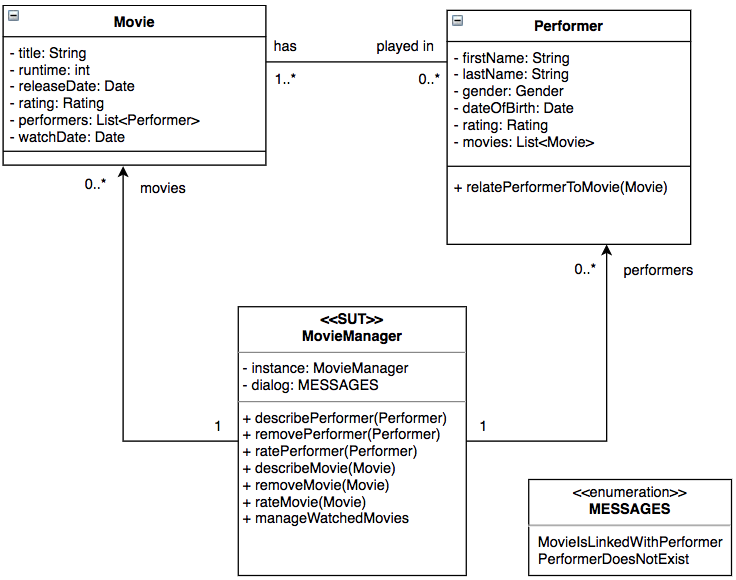
\includegraphics[scale=0.42]{../images/Ap2-class} 
\caption{Example for a class diagram of Movie Manager}
\label{fig:Ap2-class}
\end{figure}

The Movie Manager Class Diagram defines the data and the points of control and observation of the application under test. The enumeration \enquote{Messages} represents the possible message/warning to be displayed on the dialog window of the application. For our case, we considered only the messages like, \textit{movie is linked with performer} and \textit{performer does not exist}.

In addition to class diagram, an instance diagram and a state machine are also provided in the use case scenario of the provided approach. In the approach, the test generation method of LEIRIOS Test Designer consists in testing all the possible behaviors of the specification operations, by traversing the states of the system. But in our implementation, we have to skip this step since it is performed by the LEIRIOS Test Designer tool, which is called now Smartesting as already explained in ~\autoref{subsec:DE2}. We cannot use the tool right now, because it requires a scheduling even for the demo version. 

Therefore, we give only exemplarily two different internal activities specified according to the description in the article \cite{Paper2}, one for the user option \enquote{remove movie}, and other one for the user option \enquote{rate performer}, as shown in \autoref{tab:intact}. 

\begin{table} [H] 
	\begin{small}
  \begin{center}
  \begin{scriptsize}
\caption{Example of internal transitions}
\label{tab:intact}
\begin{tabular}{  m{3.3cm} | m{3.4cm} | m{6.4cm}  }
\hline
\textbf{Trigger/Label}& \textbf{Guard}&\textbf{Effect}   \\
\hline
removeMovie (movie)
\newline- Case movie is linked with a performer & Movie-$>$linked (m: movie $|$ m.linked=True) & MESSAGES\textbf{::} MovieIsLinkedWithPerformer \textbf{/*@REQ: MM-2@*/}\\
\hline
ratePerformer (performer)
\newline- Case performer does not exist & Performer-$>$exists (p: performer $|$ p.exists=False) & MESSAGES\textbf{::} PerformerDoesNotExist \textbf{/*@REQ: MM-7@*/ }\\
\hline
\end{tabular}
\end{scriptsize}
 \end{center}
\end{small}
\end{table}

These are the transitions, which are triggered by a user event, a guard and an effect. Requirements traceability is managed by tagging the effect of each transition with requirement identifiers. For example, the requirement MM-7 is used to annotate the effect in case of not existing performer. This is the link between the model and the requirement. \\
As last step, this link between the model and the requirements should be used by the LEIRIOS Test Designer tool to produce the traceability matrix between generated test cases and requirements. For each transition a test target and a test case should be via LEIRIOS Test Designer tool generated. 

Since we cannot use the tool, we generate the test cases as an example for both transitions manually. \autoref{tab:T1} and \autoref{tab:T2} presents these generated test cases for the two internal transitions showed in \autoref{tab:intact}.

\begin{table} [H] 
  \begin{center}
  \begin{small}
\caption{Test 1: Movie is linked with performer - Covered Requirements: MM-2}
\label{tab:T1}
\begin{tabular}{ m{0.8cm} | m{5cm} | m{7.3cm} }
\hline
\textbf{Step}& \textbf{Operation}&\textbf{Attributes Values}   \\
\hline
1 & MM2.removeMovie (movie)& MM2.display = MovieIsLinkedWithPerformer\\
\hline
\end{tabular}
\end{small}
 \end{center}
\end{table}
\begin{table} [H] 
\begin{center}
 \begin{small}
\caption{Test 2: Performer does not exist - Covered Requirements: MM-7}
\label{tab:T2}
\begin{tabular}{  m{0.8cm} | m{5cm} | m{7.3cm}  }
\hline
\textbf{Step}& \textbf{Operation}&\textbf{Attributes Values}   \\
\hline
1 & MM7.removePerformer (performer) & MM7.display = PerformerDoesNotExist\\
\hline
\end{tabular}
\end{small}
 \end{center}
\end{table}



\section{Comparison}
\label{sec:Compar}

In this section, we describe the special features, similarities and differences of each approaches.

Both approaches are very similar in terms of the way they use the information and of their steps. They both use informal requirements as input for their approaches, use system models for this purpose (UML models including OCL), and make use of requirements traceability for ensuring the quality of the generated test cases. They both offer tool support to generate tests automatically. 

However, there are also differences between them. In the first approach, \cite{Paper1}, the informal requirements are analyzed and structured into requirements models and then OCL is used for verifying the quality of these requirements models.
In the second approach, \cite{Paper2}, the expected functional requirements of the system under test are derived from a use case scenario. The requirements traceability is managed by tagging manually the postconditions of the operations and the effects of the transitions in the UML model with the requirements via ad-hoc comment symbols in order to associate a requirement with an OCL statement which will be involved into a test target during the generation of the test cases.

Furthermore, the LEIRIOS Test Designer tool provided in the second approach does not offer a tool support for tracing-back requirements from tests to models, while the first approach supports it via the automatically generated test report by their provided tool, Qtronic.
\newpage
\autoref{tab:TSM} presents the detailed comparison of both approaches as a synthesis matrix. In the first column, the number of the synthesis questions are presented. Number 1 implies the description, number 2 implies the benefit, number 3 implies the tools, and number 4 implies the quality for the compared approaches. Then, the second column presents the answers to these questions for approach 1, and third column for approach 2. 

\newpage
\newgeometry{margin=1cm}
\begin{landscape} 
%\begin{scriptsize}
\begin{small}
\begin{longtable}{ p{0.5cm} | p{11cm} | p{11cm} }
\caption{Synthesis matrix}
\label{tab:TSM}
\\    %%%%<===
\hline
\textbf{No.} & \textbf{Approach 1: Tracing Requirements in a Model-Based Testing Approach}  & \textbf{Approach 2: Requirements Traceability in the Model- Based Testing Process} \\
\hline
1a) & - Informal requirements
\newline - Requirements models via requirements diagram of SysML
\newline - UML Models, e.g. class Diagram specifies a domain model, a behavioral model describes the behavior of the SUT using state machines, data models describe the message types exchanged between different domain entities, domain configuration models represents specific test configurations using object diagrams.
\newline - Generated tests and test report
 & - Informal requirements
\newline - UML Models (including OCL) e.g. Use case diagram, class diagram, enumeration diagram, instance diagram, state machine.
\newline - Links between the requirements and models
\newline - Test cases and test scripts
\newline - Traceability Matrix \\
\hline
1b) & Informal requirements are input for this approach.
\newline A set of modeling guidelines and validation rules should also be defined.
\newline In order to automatically transform UML models to the QML via the Qtronic tool, all requirements should have been linked to model elements and the models should have been validated.
\newline The desired coverage criteria used for test generation should be manually selected from the GUI of Qtronic.
\newline The presented approach is for functional requirements and it only supports online testing. & Informal requirements are input for this approach. 
\newline Uncontrollable or unobservable elements should not be modeled.\\
\hline
1c) & 1. The informal requirements are analyzed and structured into a requirements model using the requirements diagrams of the SysML.
\newline 2. SUT is specified using UML (including OCL) and several perspectives of the SUT are modeled, e.g. class diagram, behavioral model, data models, domain configuration models etc. 
\newline 3. A set of modeling guidelines and validation rules are defined using OCL. MagicDraw tool has been used for editing the SysML and UML models and for running the validation rules
\newline 4. The models used to specify the SUT are subsequently transformed into input for the automated test derivation tool Qtronic. 
\newline 5. At the end of each test run, an automatically generated test report will summarize the result of the testing process in terms of generated test cases, verdicts, coverage levels etc.
& 1. UML-Modelling of functional requirements of the application under test, e.g. class diagrams, instance diagrams, state machine diagrams  etc.
\newline2. Tagging manually the post-conditions of the operations and the effects of the transitions in the UML model with the requirements. The format uses ad-hoc comment symbols in order to associate a requirement with an OCL statement which will be involved into a test target during the generation of the test cases.
\newline3. Driving the test generation process in which the generation of tests is steered by the validation engineer on the basis of test selection criteria.
\newline4. Test generation method provided by the LEIRIOS Test Designer tool
\newline5. Executable test script generation which are converted from the generated test cases via LEIRIOS Test Designer. A test script pattern and a mapping table are to be defined by the test engineer.\\
\hline
2a) & Test generation, and tracing requirements to models, to test specification, and back to models again.& Test generation, and tracing requirements to test cases. \\
\hline
2b) & Product engineer, software engineer, requirement engineer and user of the provided tooll/tester.  & Validation engineer, software engineer, requirement engineer and user of the provided tool/tester. \\
\hline
2c) & Chapter 1: Software Requirements
\newline - Requirements Process
\newline - Requirements Analysis
\newline - Practical Considerations (e.g. Requirements Tracing)
\newline Chapter 4: Software Testing
\newline - Test Techniques (e.g. Model-Bases Testing Techniques)
\newline -  Software Testing Tools (e.g. Testing Tool Support and Categories of Tools)
\newline Chapter 9: Software Engineering Models and Methods 
\newline - Modeling
\newline - Types of Models
\newline - Analysis of Models (e.g. Traceability) & Chapter 1: Software Requirements 
\newline - Requirements Process (e.g. Process Actors)
\newline - Requirements Analysis
\newline - Practical Considerations (e.g. Requirements Tracing)
\newline Chapter 4: Software Testing
\newline - Test Techniques (e.g. Model-Bases Testing Techniques)
\newline -  Software Testing Tools (e.g. Testing Tool Support and Categories of Tools)
\newline Chapter 9: Software Engineering Models and Methods 
\newline - Modeling
\newline - Types of Models
\newline - Analysis of Models (e.g. Traceability) \\  
\hline
3a) & The NoMagic’s MagicDraw has been used for editing the SysML and UML models and for running the validation rules. \newline Conformiq’s Qtronic tool is provided for the automated test derivation and test report generation. Only online testing mode of Qtronic is used to generate tests. & LEIRIOS Test Designer tool is provided to generate test cases and to produce the traceability matrix between generated test cases and requirements. The tool is used in the test and test script generation processes.\\
\hline
3b) & The creation of the models is not automated and the desired coverage criteria used for test generation should be manually selected from the GUI of Qtronic. Tests and test reports are automatically generated by the provided tool, Qtronic. &Requirements traceability is managed by tagging manually the postconditions of the operations and the effects of the transitions in the UML model with the requirements via ad-hoc comment symbols. Tests are automatically generated by the provided tool, LEIRIOS.\\
\hline
4a) & Approach does not present an evaluation. Only validation rules have been defined and implemented for both requirements models and for SMs for checking different quality metrics of the resulting models before proceeding to the test derivation phase.
\newline For the description of the approach, only small examples from a telecommunications case study are provided. & Approach does not present an evaluation. Only for a simpler description, the approach is implemented on a simplified version of a drink vending machine controller.\\
\hline
4b) & Since the approach does not offer any evaluation, only the benefits and shortcomings of the approach have been shared as below:
\newline - The approach provides a solution for tracing only functional requirements and supports only online testing.
\newline - The approach provided automation of the transitions between the phases of the process, allowing to have a fast feed-back loop for testing and debugging specifications or the implementation of the SUT.
\newline - Many errors have been detected in the early stages of the process, when the system models have been created. The errors were caused mainly by omissions in the models and by misinterpreting the requirements.
\newline - Since the approach is fully automated, the effort in updating the models and performing the testing again was diminished.
 & Since the approach does not offer any evaluation, only the benefits and shortcomings of the approach have been shared as below:
 \newline - Automatically produced traceability matrix leads to several advantages in the software testing process, e.g. it gives a clear functional coverage metrics to the generated test cases, enables to improve the model or test generation strategies, and gives valuable feed-back on the requirements.
 \newline - There is no tool support for tracing-back requirements from tests to models.\\
\hline
\end{longtable}
\end{small}
%\end{scriptsize}
\end{landscape} 
\restoregeometry


\newpage
\section{Conclusion}
\label{sec:Conc} 
This chapter presents two approaches for the testing with system models. Both approaches, \cite{Paper1} and \cite{Paper2}, use requirements traceability in their model-based test generation processes and provide a tool support to generate tests automatically. 

The literature research showed us that the for this topic relevant articles are mostly published between 2000-2009. Although there are a lot of articles which provide approaches based on the links (traces) between requirements and test cases, only a few of them are using system models. Therefore, it is important to differentiate the system model and test model with respect to the model-based testing. However, based on our research, we could not find a sharp difference between the two. Our conclusion is that test models are developed solely for testing while system models can be primarily developed for system development and then used for testing as well. Moreover, with this literature study, we came to the conclusion that it is laborious to find relevant articles with keyword-based search method, because requirements traceability and model-based testing are very comprehensive topics in Software Engineering. 

The first approach studied in this chapter, \cite{Paper1}, describes the MBT process in more detail than the second approach \cite{Paper2} does. But \cite{Paper2} presents a more detailed use case example with more visuals which enables us to understand the steps of the testing process better. However, both approaches lack the detailed explanation on how the test cases are generated via the provided test generation tools. For the generation of test cases, \cite{Paper1} provided Conformiq's Qtronic tool, which is unfortunately not existing anymore, and \cite{Paper2} provided the LEIRIOS Test Designer tool, which is named currently Smartesting. Therefore, we could not find the necessary information on how these tools implement the test generation step in practice. Unfortunately, no evaluation was offered for either approach. All of this makes it difficult for us to make an accurate assessment between these two tools/approaches. In our opinion, if we had to choose one of this approaches, it would make more sense to choose the second approach \cite{Paper2}, as LEIRIOS Test Designer tool (Smartesting) is still on the market. It has probably evolved over the ten years as well.

Finally, both approaches presented in this chapter showed us that testing with system models enables to increase the possibility of finding errors, reduce the testing time, and improve the test quality using requirements traceability.
